% Results and Discussion

% Chapter Template

\chapter{Results and Discussion} % Main chapter title

\label{Results and Discussion} % Change X to a consecutive number; for referencing this chapter elsewhere, use \ref{ChapterX}

%\lhead{Chapter 1. \emph{Introduction}} % Change X to a consecutive number; this is for the header on each page - perhaps a shortened title

\renewcommand{\chaptermark}[1]{\markboth{#1}{}}
\renewcommand{\sectionmark}[1]{\markright{#1}}
\fancyhead[RE]{\small\leftmark}
% Section in the left on even pages}
\fancyhead[LO]{\small\rightmark}%Section in the left on odd pages

%\section{A section goes here}

%A figure

\textbf{Balancing noise removal and sparsity of component abundance dataset}\\

The ecological analyses in this thesis started with two datasets of component counts from the TARA ocean prokaryotic metagenomes from all depths (TP) and only the surface samples (TPS). These two datasets were filtered first for low total count samples (Methods: Initial dataset preparation) and second for low mean proportion components. This ensured that: (1) extremely low abundant components were filtered out; (2) sequencing noise was removed; and (3) overall size of the resulting abundance matrices was decreased to lower computational resources for calculations.

\begin{figure}[h!]
	\centering
	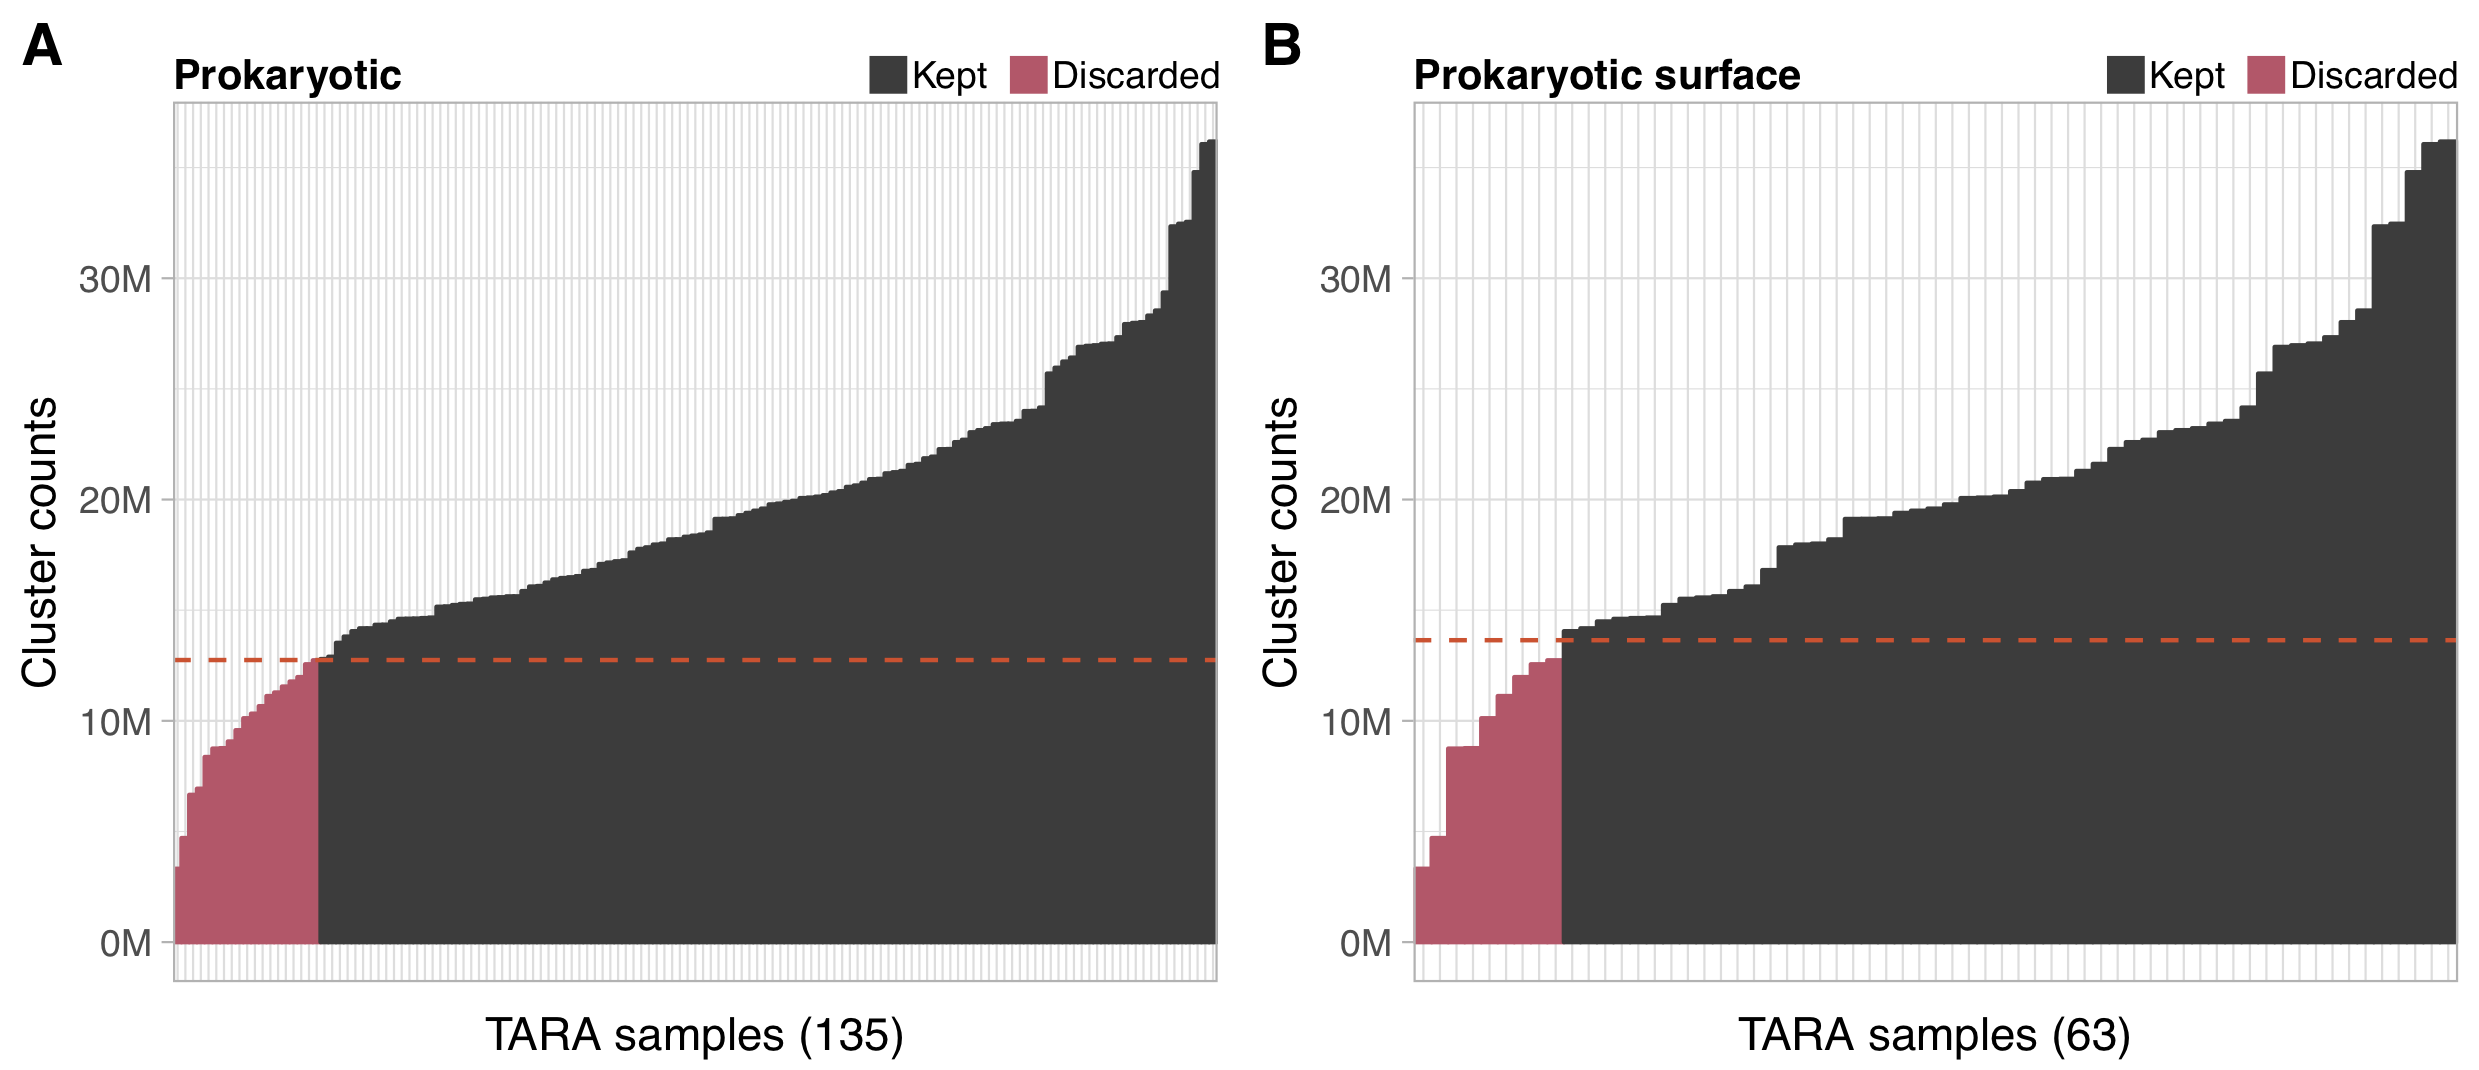
\includegraphics[width=1.0\textwidth] {fig_2}
	\caption{\textbf{Step 1 of dataset filtering.} X axis denotes each sample in the dataset while the Y axis denotes total cluster counts for each sample. Samples with total counts below the median subtracted from 1.5 multiplied the MAD were removed from the analyses.(A) Total component counts for TARA prokaryotic metagenomes (TP). (B) Total component counts for TARA surface, prokaryotic metagenomes (TPS).}\label{fig2}
\end{figure}

During the first filtering step, nine samples were removed from the TPS dataset and 19 samples were removed from TP dataset. Sample with low total counts, relative to other samples, have the potential to distort beta-diversity analysis because their total counts could make them more similar to each other due to low counts rather a real beta-diversity signal. The Median - 1.5*MAD (median absolute deviation) cutoff threshold was chosen because the MAD statistic was chosen it is a reliable measurement of the center of the data and is not sensitive to outliers (Fig. 3.1). \\

The second filtering step removed all components that had a mean proportion across all samples lower than 1e-5. After this step, the final TPS dataset contained 18,644 components while the TP dataset contained 15,353 respectively. This was an effective cutoff for both the TP and TPS datasets because overall component content and counts were able to be maximized while sparsity was lowered. The less sparsity an abundance table has, the more power the abundance variables have in explaining the dataset. Yet, a side effect of decreasing sparsity is removing counts which decreases the total amount of information the dataset has. In both datasets, if the mean proportion requirement was increased to 1e-4, sparsity would have reached close to 0. This could have led to a large amount of total counts and components being sacrificed. For this analysis, we did not want to remove the low abundance signals in order to capture more functional diversity in the dataset. A summary of the different mean proportion used can be seen in Fig. 3. \\

\begin{figure}[h!]
	\centering
	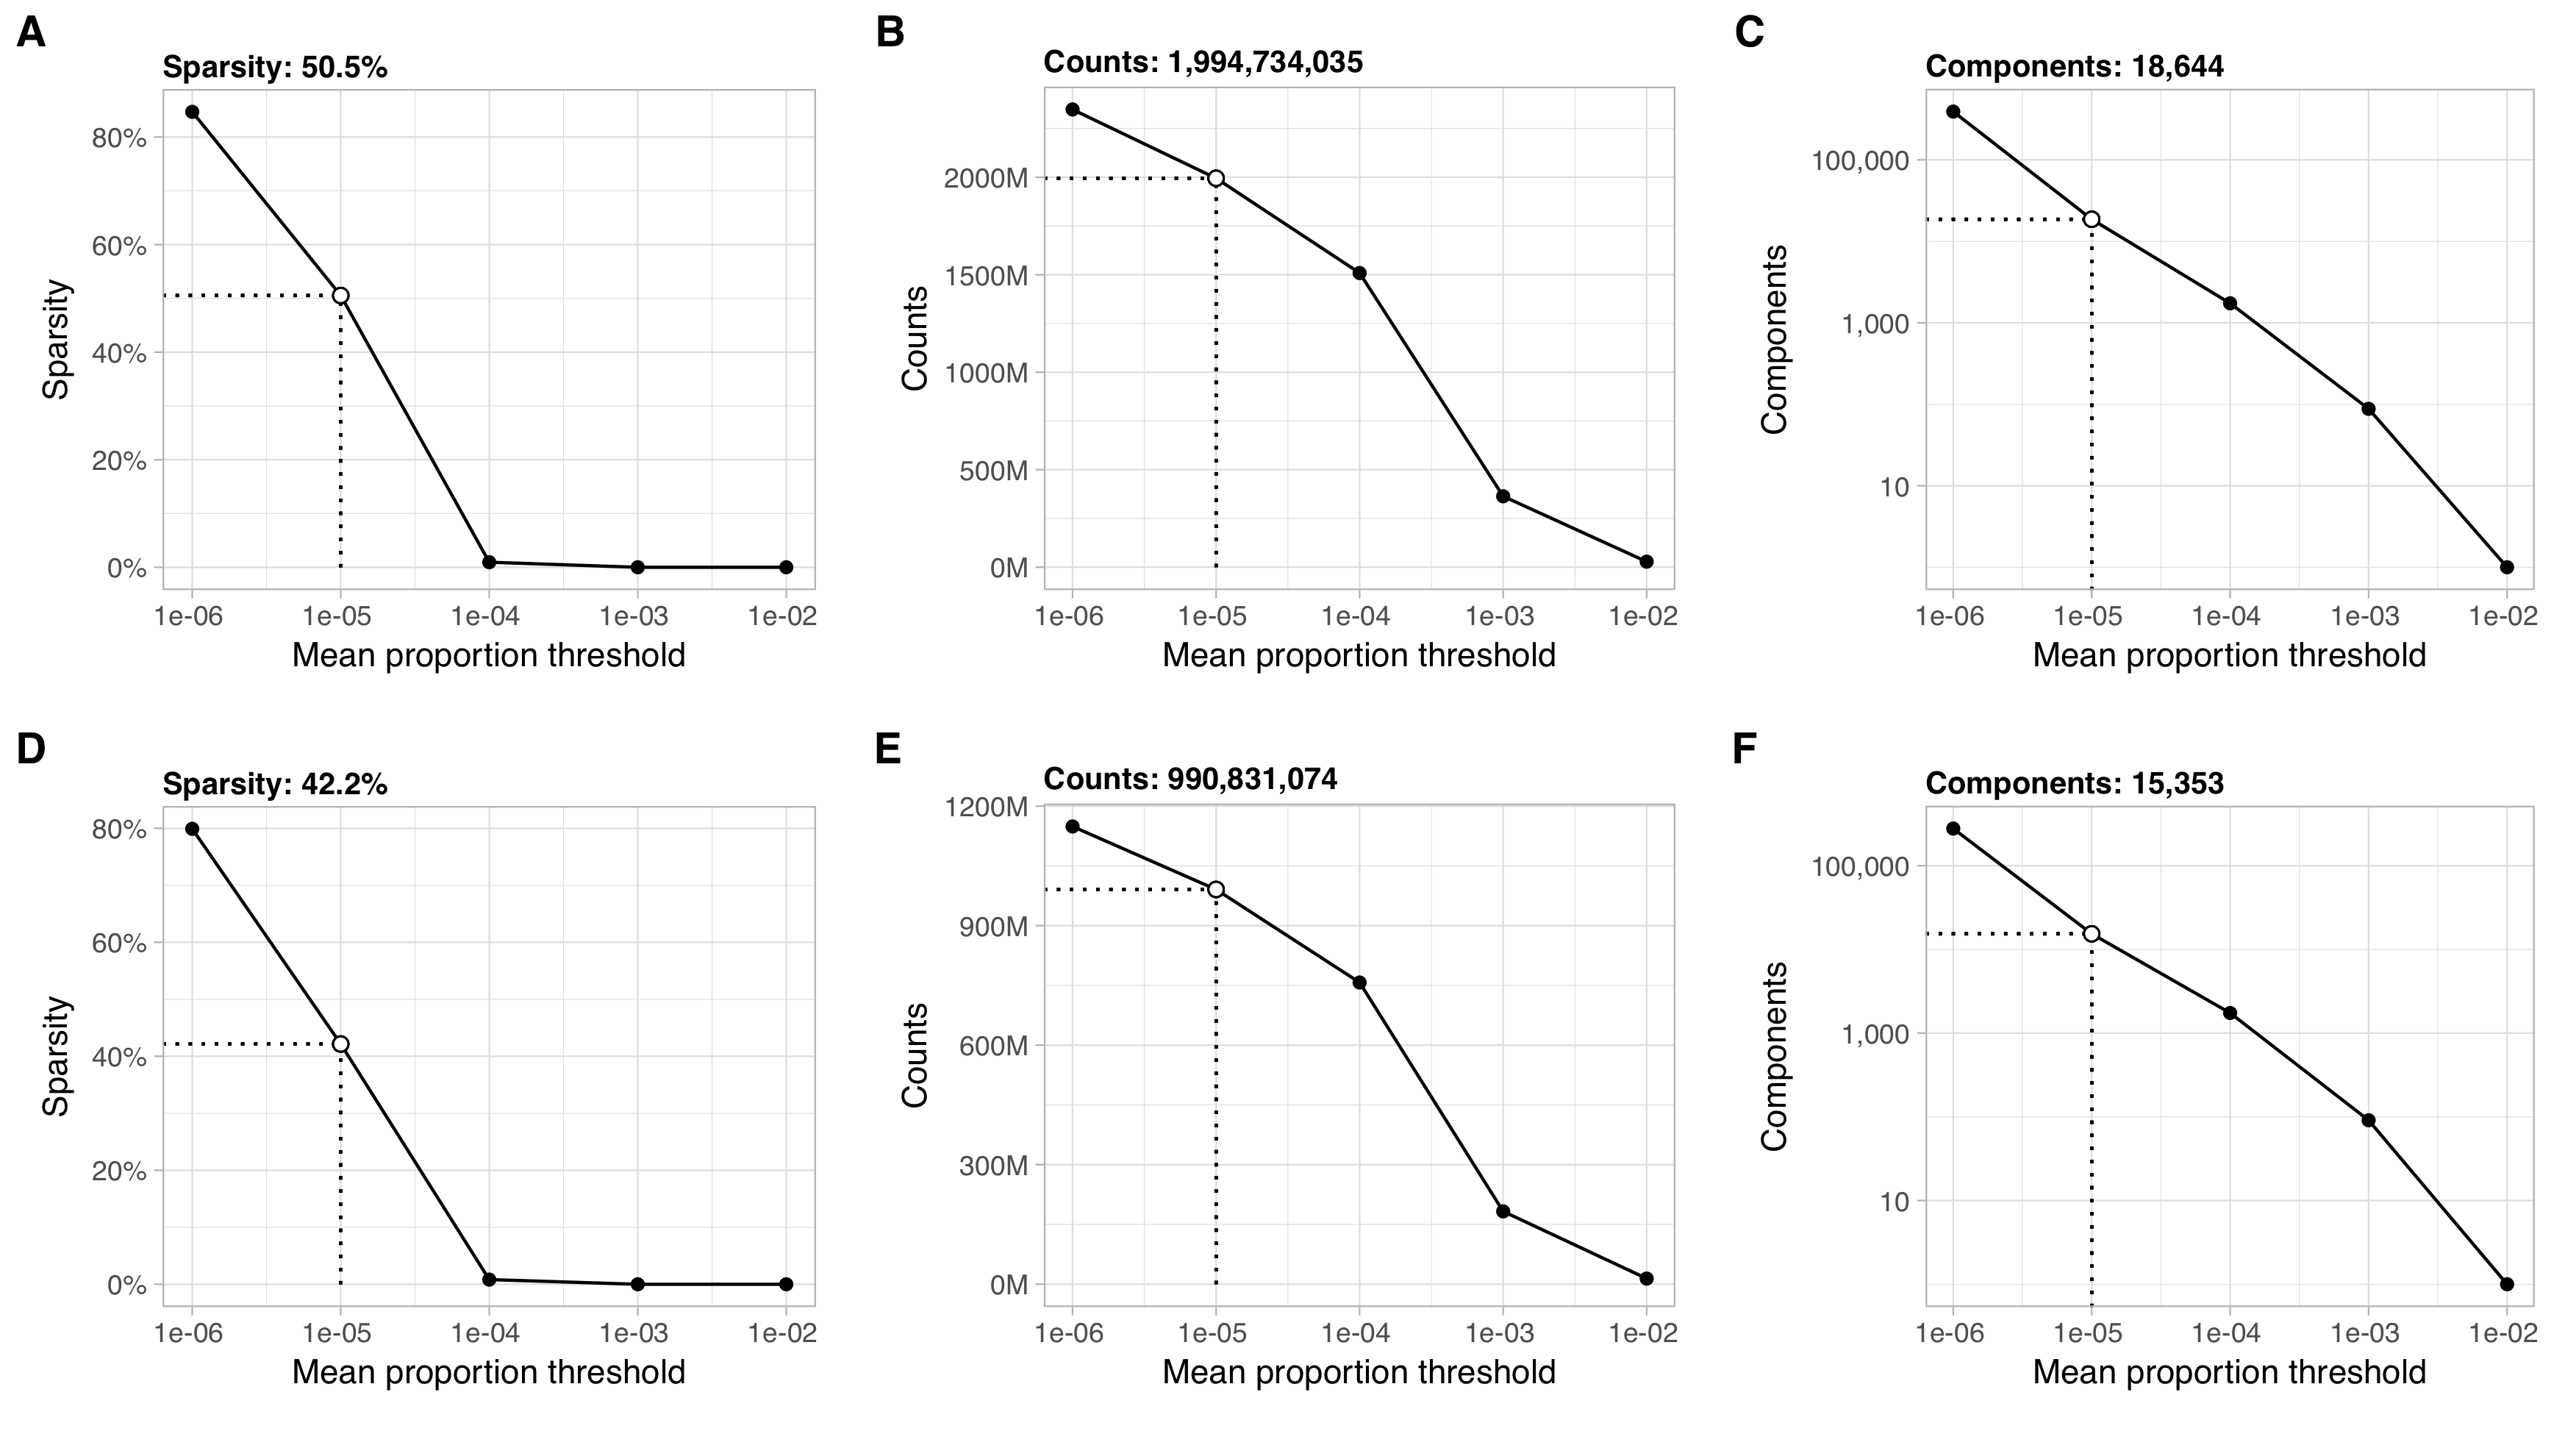
\includegraphics[width=1.0\textwidth] {fig_3}
	\caption{\textbf{Metagenome component mean proportion (1e-5 cutoff) plotted against dataset sparsity, total cluster counts, and number of components.} Caption: A-C represents the TARA prokaryotic, all depths dataset (TP). D-F represent the TARA prokaryotic, surface dataset (TPS).}\label{fig3}
\end{figure}

\textbf{Indirect gradient analysis of TARA Ocean sites based on component abundances}\\

\begin{figure}[h!]
	\centering
	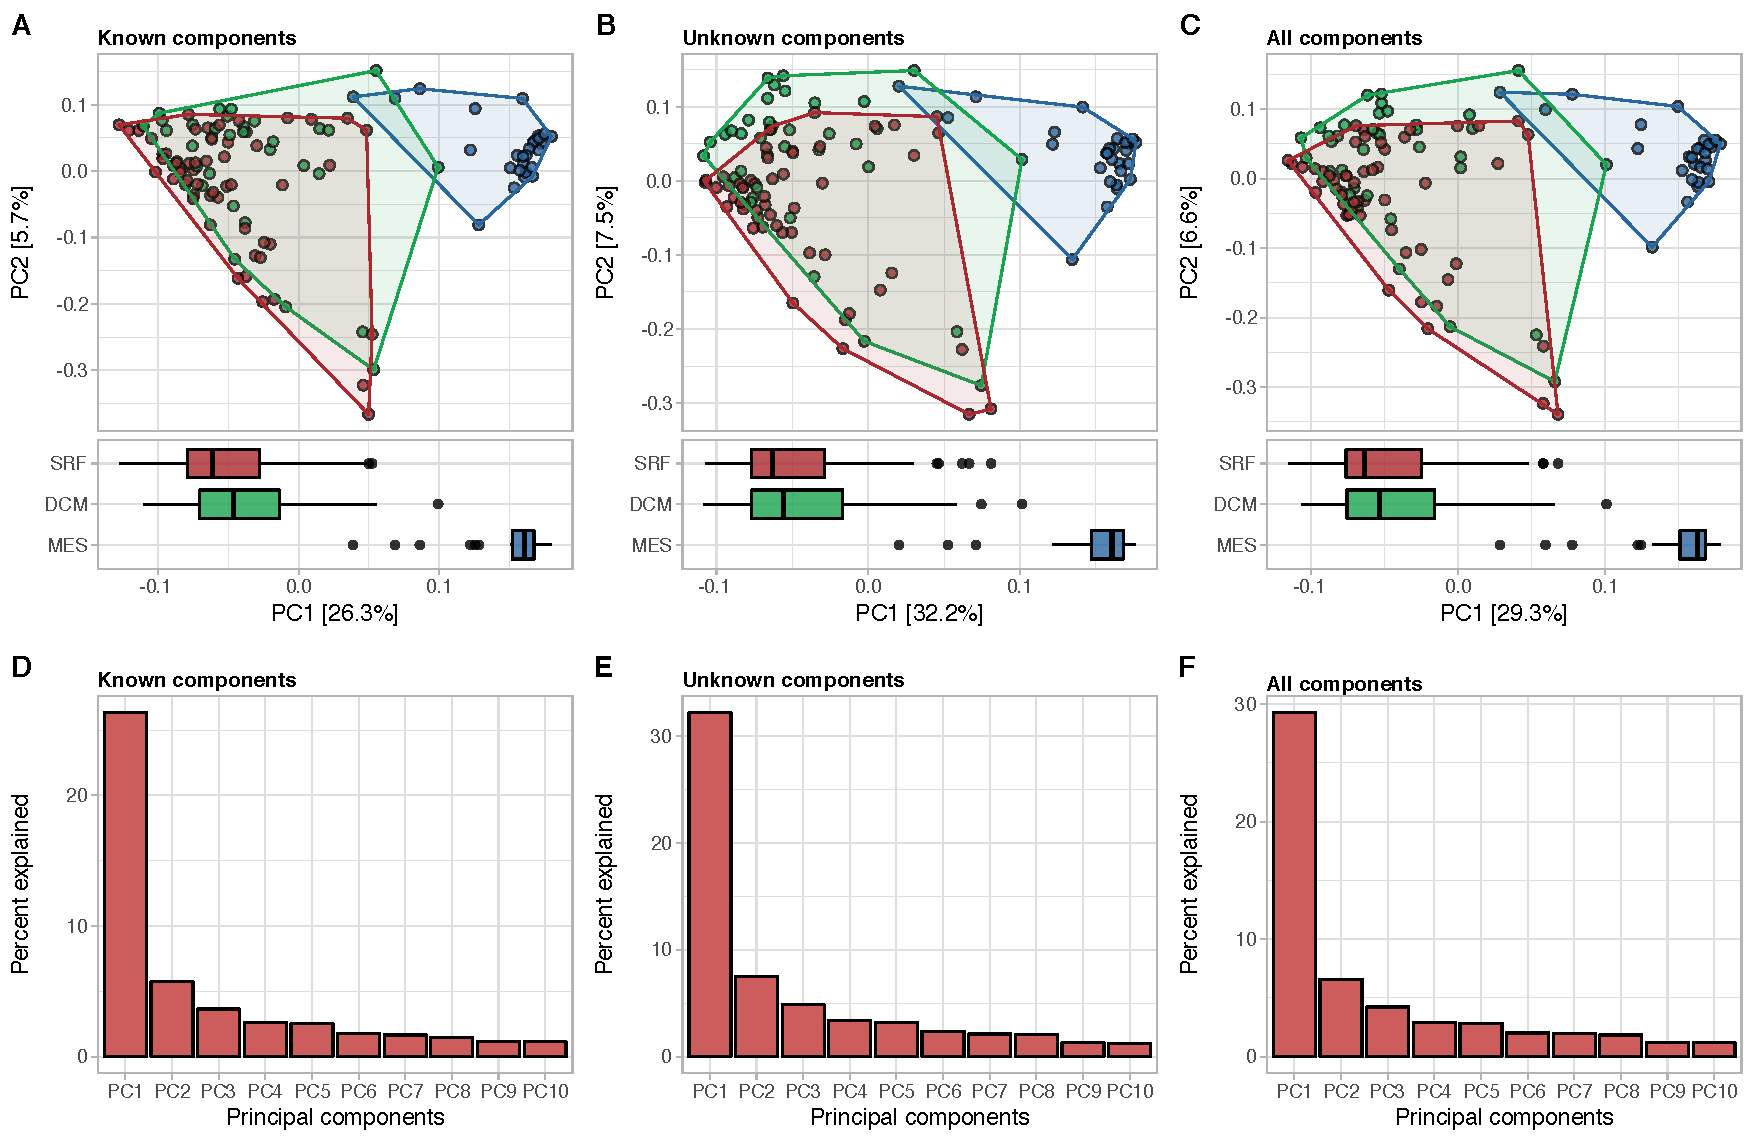
\includegraphics[width=1.0\textwidth] {fig_4}
	\caption{\textbf{Principal component analysis (PCA) of 135 TARA Ocean prokaryotic metagenome sampling sites from surface (SRF), deep chlorophyll maximum (DCM), and mesopelagic (MES) sites} A-C) Sites are colored by depth of origin are defined by proportions of component categories: Unknowns (EU + GU), Knowns (K + Kwp), All (EU + GU + K + Kwp). Below each ordination are bar plots of the distribution of each component category across the first principal component axis. D-F) Scree plots of each PCA. The X axis denotes each principal axis while the Y axis denotes the percent variance explained by the axis. Residuals of each PCA ordination can be found in the supplementary materials Fig . S2}\label{fig4}
\end{figure}

Principal component analysis (PCA) of the TARA ocean prokaryotic sample sites produced a meaningful ordination (Fig. 3.3 A-C). Due to the effect of compositionality often associated with ?omics datasets, a center log ratio transformation (CLR) was performed prior to calculated the PCA \citep{Gloor_2017}. Scree plots indicated that in all three ordinations the majority of variance was captured in the first two principal component axes (PC) (Fig. 3.3 D-F). Additionally, histograms of residuals were calculated and showed a bimodal distribution (Fig. S1). NMDS ordination was calculated using pairwise site Bray-Curtis dissimilarity (Fig. S2). The calculation was iterated 20 times with a stress ~ 0.8 for all categories (Table 3.1).

\begin{table}[]
\centering
\caption{Stress Values for NMDS ordination}
\label{my-label}
\begin{tabular}{ll}
\textbf{Component Category}   & \textbf{NMDS stress} \\
\textbf{Unknowns (EUs + GUs)} & 0.07997218           \\
\textbf{Knowns (K + Kwp)}     & 0.08218745           \\
\textbf{All combined}         & 0.07974366          
\end{tabular}
\end{table}

\section{TARA Ocean Sites cluster based on depth}\\

PCA ordinations of the TARA ocean prokaryotic sample sites clustered based on their depth of origin (surface (SRF), deep chlorophyll maximum (DCM), and mesopelagic (MES) regardless of which component category sites are defined by. The SRF and DCM sites overlap, while the MES samples form their own cluster. Additionally, in all cases the first principal component axis (PC1) explains the most variance in the ordination. PERMANOVA of the ordination against the depth categories and temperature from the associated metadata was significant, allowing the rejection of the null hypothesis that the three depth categories have the same cluster centroids in the ordination (Table 6). Additionally, beta-dispersion was not significant for the depth category indicating that clustering was not due to dispersive effects. If beta dispersion was significant, it would indicate that clustering of sites in the ordination was due to dispersion effects of the data and not entirely due to contextual data. But it was not significant, there is increased confidence in the PERMANOVA. NMDS ordination based on Bray-Curtis dissimilarity also show the same clustering of sites based on depth category and temperature (Supplementary Materials Fig. 13). \\

\begin{table}[]
\centering
\caption{TARA ocean prokaryotic metagenome sampling site ordination due to temperature hypothesis testing}
\label{my-label}
\begin{tabular}{lll}
\textbf{Component Category}   & \textbf{PERMANOVA R\textasciicircum 2} & \textbf{p-value} \\
\textbf{Unknowns (EUs + GUs)} & 0.21144                                & 0.001            \\
\textbf{Knowns (K + Kwp)}     & 0.17109                                & 0.001            \\
\textbf{All combined}         & 0.19232                                & 0.001           
\end{tabular}
\end{table}

Previous ordinations of the TARA Ocean metagenomes have shown site clustering by depth of origin (Sunagawa et al., 2015; Louca et al., 2016). Louca et al., calculated a metric multidimensional scaling (MDS) of the TARA sampling sites, but instead, defined sites based on aggregated, biogeochemically relevant microbial functions. Additionally, Sunagawa et al. and Louca et al. calculated a principal coordinate analysis with sites defined by 16S rDNA gene tags (miTAG) extracted from the metagenomes. Both analyses concluded that prominent environmental factors (e.g. temperature, nutrients levels, access to light) from the different depth layers have a strong influence in shaping the structure and function of the microbial community. This explanation can be applied to this analysis as well.

\begin{table}[]
\centering
\caption{TARA ocean prokaryotic metagenome sampling site ordination due to depth category hypothesis testing}
\label{my-label}
\begin{tabular}{llll}
\textbf{Component category} & \textbf{PERMANOVA R\textasciicircum 2} & \textbf{p-value} & \textbf{Beta dispersion p-value} \\
Unknowns (EUs + GUs) & 0.27237 & 0.001 & 0.073 \\
Knowns (K + Kwp) & 0.22649 & 0.001 & 0.121 \\
All combined & 0.25064 & 0.001 & 0.117
\end{tabular}
\end{table}

Regardless of what cluster category an ORF is from, the environmental factors from the depth layer are selecting components in a similar way. The SRF and DCM samples may overlap due to depth proximity. Both SRF and DCM are sunlit environments and have access to fresh primary production carbon sources. On the other hand, the MES samples clusters separately from the SRF and DCM. This is most likely owing to the different environmental factors in the MES, such as lack of solar radiation, lower temperatures, and higher dissolved oxygen and nutrients, which can select for different microbial functions than the epipelagic depths. Additionally, there is increased amounts of recalcitrant carbon sources in the MES because smaller/simple carbohydrate sources are most likely respired at high depths of the biological carbon pump \citep{Azam_2007}. In an environment with more complex carbon sources, a diverse array of microbial functions may be selected for to metabolize a wider range of carbon sources.\\

\textbf{Increased variance when the whole metagenome is accounted for}\\

In Fig. 4 A-C, more variance is captured in PC1 of the Unknowns (32.2\%) while less variance is captured in the Knowns PC1 (26.3\%). The Knowns + Unknowns PC1 variance falls in between (29.3\%). The fact that PC1 of the Unknowns ordination has the most variance infers that sites are more dissimilar when they are defined by the unknown fraction of components. Also, by accounting for both the Known and Unknown fraction in the All ordination, the site dissimilarity is effectively increasing by including the Unknown fraction. 
Similar to defining sites with all detected OTUs regardless if taxonomy is assigned to them, ORF clusters, with or without annotation, can be tracked as a functional entity in metagenomes and help separate samples in higher resolution. Louca et al., 2016 ordinated the TARA Ocean sites based on biogeochemical relevant microbial functions and determined there was functional redundancy in the ocean. This conclusion may have been constrained by the fact that sites were only defined by known functions. If the Louca et al., 2016 sites were defined with the complete functional repertoire of the metagenomic sample, their results may have had increased dissimilarity. It is clear that when sites are defined by the knowns and the unknowns, more variance is added to the ordination. This may indicate that the unknown fraction could be site specific adaptive proteins. \\

\textbf{Unique component composition in Southern Ocean Samples}\\

\begin{figure}[h!]
	\centering
	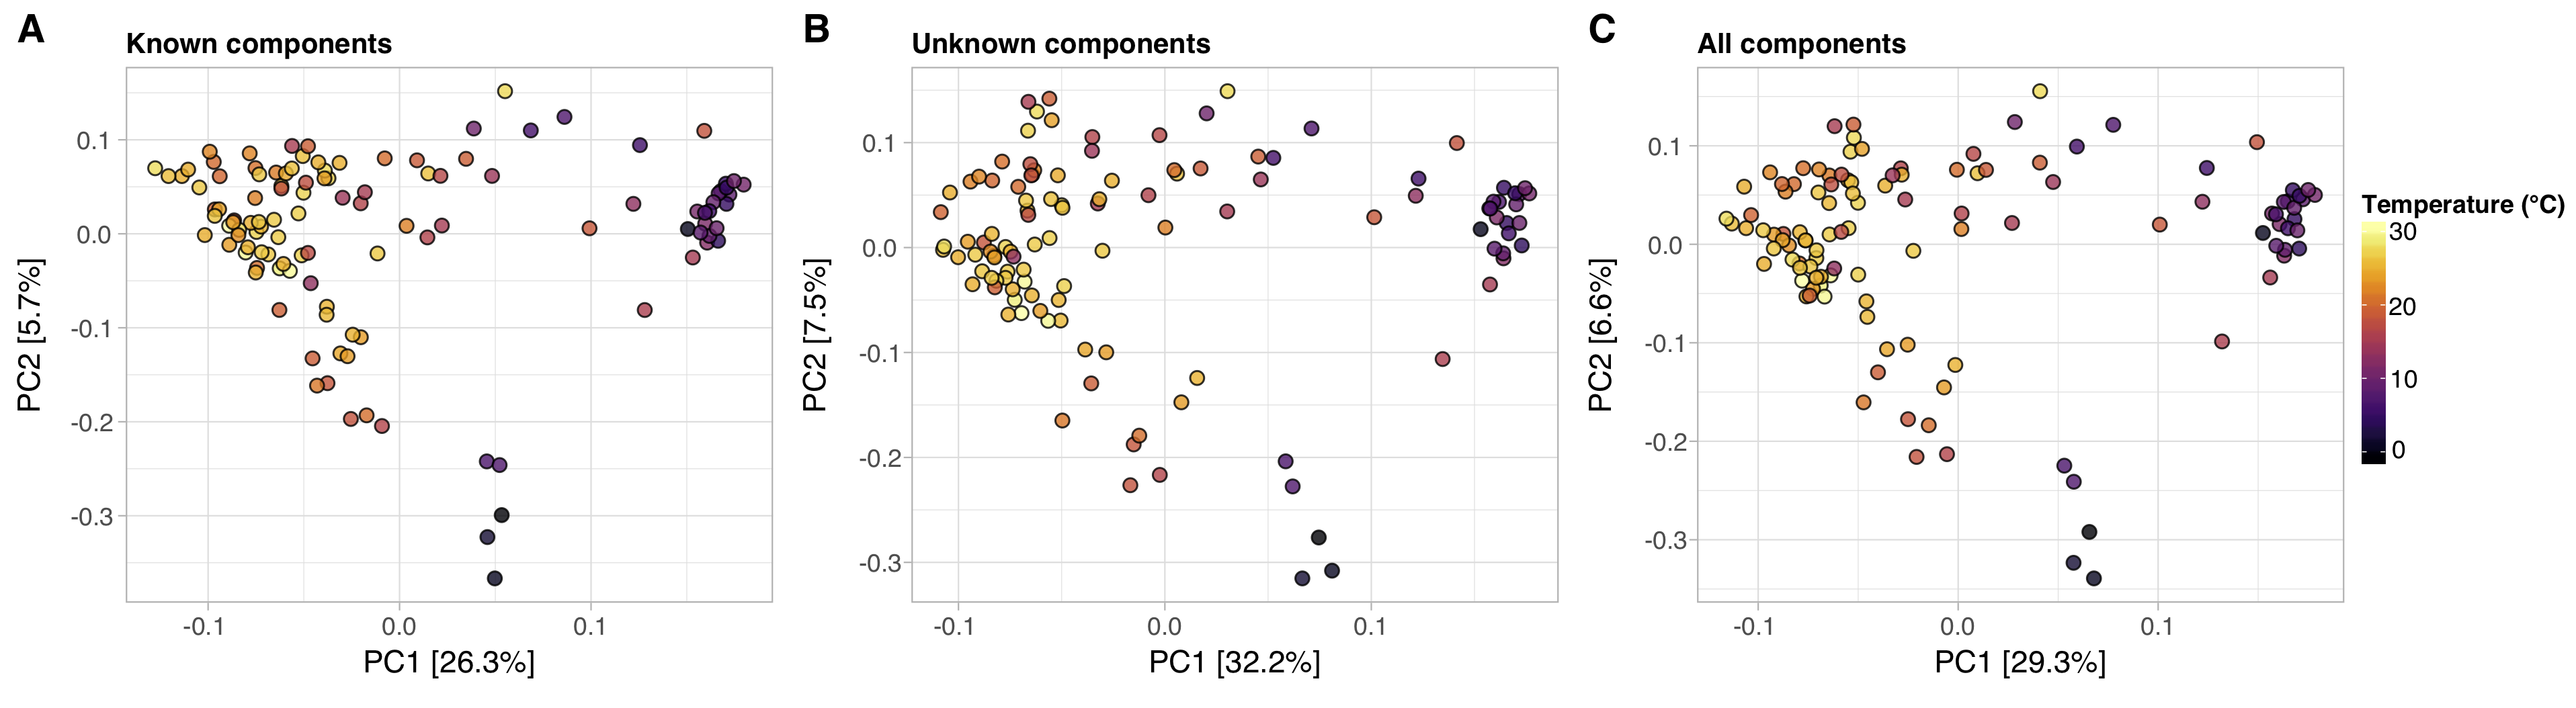
\includegraphics[width=1.0\textwidth] {fig_5}
	\caption{\textbf{Principal component analysis of the prokaryotic fraction of the 139 TARA ocean sampling sites from all depths colored by temperature}}\label{fig5}
\end{figure}

A temperature gradient across PC1 of Figures was ordinated in the TARA sampling sites. Samples in the SRF and DCM cluster have warmer temperatures while the MES cluster has the coldest temperatures. Colder samples from the SRF and DCM ordinate closer to the MES cluster. These results are in line with Sunagawa et al., 2015 who found that temperature is the main driving factor for community composition in the ocean. The SRF and DCM have warmer temperatures due to increased solar radiation, while heat is dissipated in the MES. The clustering of the ordinations based on the origin depth of the sample may be due to temperature which could then select for different microbial functions (PERMANOVA for temperature found in table 4). \\

An exception to the temperature gradient across PC1 are the three Southern Ocean samples (TARA site 84 SRF, DCM and site 85 SRF) at the bottom of the ordination. Even though they are some of the coldest samples in the dataset, they do not follow the temperature gradient along PC1 and do not cluster with the rest of the cold MES samples. In fact, PC2 appears to drive their separation from the rest of the samples. \\

These three Southern Ocean samples may have a unique component composition due to their placement in the Antarctic Circumpolar Current (ACC). The ACC is a located in the Southern Ocean and presents a unique biome compared to other oceanic currents due to its strength, isolation, dramatic seasonal light flux and nutrient levels. Strong westerly winds around Antarctica drive the current due to pressure gradients caused by surface wind friction and density differences. Because no continents obstruct its flow, the ACC is the only ocean current system that circles the earth on a similar latitude range. This allows to be the fastest current in the ocean with speeds around 130 e6 m3/s-1 through Drake passage (MarMic Physical Oceanography Lecture, 2017).\\

The ACC also has unique physicochemical properties that may also influence specialized microbial functions. Due to low altitude wind cells, Aeolian dust input is limited which makes mineral concentrations limited. On the other hand, strong upwelling increases concentrations of other nutrients, such as nitrate and phosphate. This makes for a unique environment because despite high nutrients, chlorophyll levels are low due to Fe limitations \citep{Martin_1990, Tagliabue_2014, Cavicchioli_2015}. Additionally, the ACC has unique biogeography due to dramatic polar light cycles. During summer season, long periods of light generate high levels of primary production, while during low light winter's, the overall microbial community switches to different ecological strategies such as heterotrophy and predation \citep{Wilkins_2013, Milici_2017}. Due to the reasons listed above, unique functions for local adaptation in the Southern ocean may be driving the dissimilarity from the other TARA ocean samples.\\

Interestingly, TARA site 85 MES metagenome did not cluster with the Antarctic SRF and DCM metagenomes at the bottom of the ordination, but rather clustered with the rest of the MES metagenomes. This reinforces that the MES is a different environment compared to the SRF and DCM. Even though TARA site 85 MES was sampled in the ACC, the deep depth layer environmental parameters have a stronger influence on its component composition. To further explore this observation, direct gradient analysis should be applied to the Southern Ocean to resolve its unique microbial functional properties.\\

Using sites to ordinate the TARA ocean sites revealed a distinct functional difference between the Southern Ocean samples and the rest. This was in part due to the use of components to define sites. No matter which category of components was used (Knowns, Unknowns, All), the Southern Ocean samples we separated. This is an indication that defining sites based off of component composition may help resolve fine differences between sites in ecological analyses. \\

The ordination of sample sites based on the different component fractions preliminarily indicated that the Unknown fraction may be able to increase site dissimilarity. To investigate further, we performed a Levin\textquotesingle s Niche Breadth analysis to explore component niche occupancy.\\

\textbf{Niche Breadth}\\

According to \cite{Levins_1966}, Niche breadth (B) is the theoretical, multidimensional range of resources and habitats a species can occupy and access. Here we used the equation 1 to quantify the niche specialization of all prokaryotic components in the TARA oceans sampling sites. B was originally designed to classify macro-ecology abundance biogeography, i.e. birds and deer in different environments. Ocean microbial systems are different compared to  macro-ecological systems for a few reasons. First, the definition of species in microbial ecology is still debate. Second, microbes are subjected to functional and physiological plasticity due to horizontal gene transfer. With these factors in mind, the Niche Breadth measurement is still informative for analyzing the distribution of components. Recently, the measurement was used to describe the biogeography of operational taxonomic units (OTUs) in coastal Antarctic lakes \citep{Logares_2012}. \cite{Logares_2012} used B to denote ?generalists? vs ?specialists? to explore niche specialization of microbes within the domain of the sampling regime. It has also been hinted that the distributions and associations of genes with ecological niches may be an effective strategy for determining the role of accessory/adaptive genes in pangenomic diversity \citep{Shapiro_2017}. Although more studies need to be done, these studies have laid groundwork for using Niche Breadth in the context of component distribution. \\ 

\begin{figure}[h!]
	\centering
	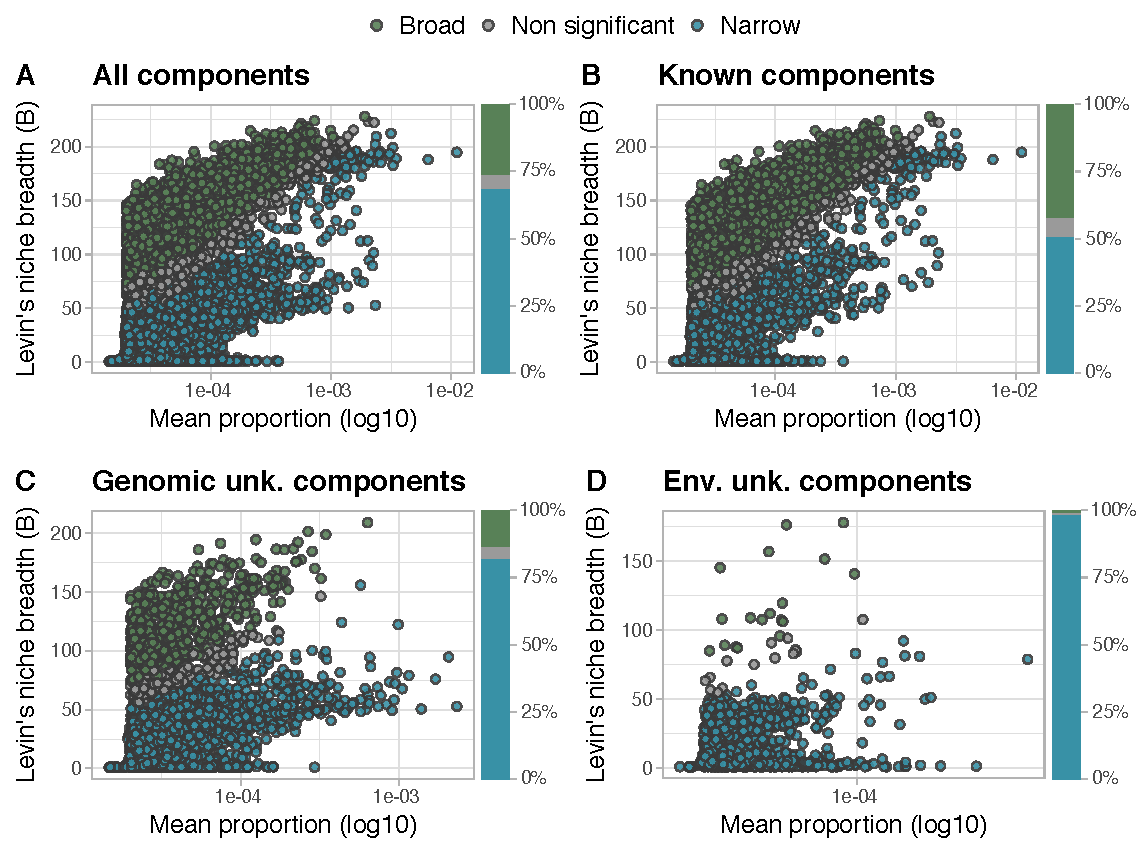
\includegraphics[width=1.0\textwidth] {fig_6}
	\caption{\textbf{Levin\textquotesingle s Niche Breadth (B) scores of the component categories.}The x-axis denotes the average, relative abundance of a component across all TARA prokaryotic metagenomes. The y-axis denotes a component B scores. Components are colored by their classification due to their B score. The bar charts on the right of each plot represent the relative proportion each B classification in the component category. Components with a B that fell above the 95\% confidence interval of their distribution are classified as wide B, while components with a B that fell below the 5\% confidence interval of their distribution are considered to have a narrow niche breadth}\label{fig6}
\end{figure}

This niche breadth analysis revealed that greater than 99\% of the EU components have a narrow niche breadth. Also, the majority of GUs are narrow while the Knowns are more evenly distributed between narrow and wide components. In the sample site ordination, it was found that including the Unknown fraction increases variance between sites. This result compliments the Niche Breadth analysis because the majority of the GU and EU components are categorized as having a narrow B (i.e. found in a few samples in higher proportions). EUs in general being associated with narrowness may indicate that they are selected in prokaryotic genomes due to specific environmental factors that occur in niche spaces (TARA ocean sampling sites). These components may be uncharacterized EUs because they are non-core, accessory functions from members of the rare biosphere \citep{McInerney_2017}. Functions from the rare biosphere are difficult to characterize due the inability to culture members and assemble their genomes into metagenomic assembled genomes due to low read coverage. \\

In Fig. 6 D, there is a group of EU components that are narrow and with mean proportions greater than 1e-4. This indicates that they are found in relatively high abundance in only a few samples. These components may be truly adaptive and could be providing the microbes with a selective advantage. Additionally, in Fig. 6 B and C, there are Known and GU narrow components with mean proportions greater than 1e-3. These components may also be adaptive components and could be immediately investigated due the Knowns having a Pfam annotation and the GUs being associated with taxonomy.\\

Though taxonomy and functional annotations are not available for the EUs by definition, the niche breadth analysis still provides more evidence that they are environmentally adaptive proteins in microbes that have be selected for by specific niche factors at the site. To increase evidence for this hypothesis we examined the component categories from a biogeographical point of view. \\

\textbf{Beta diversity analyses}\\

Microbial distance-decay analysis regresses genetic distance against geographical distance between sampling sites. The general hypothesis for this analysis is that sites will increase in genetic dissimilarity (beta-diversity) with increasing distance. Here we perform a distance-decay analysis while defining beta diversity by different component categories: Unknowns (EU + GU), Knowns (K + Kwp), and All (Known + Unknown). \\

The results of distance-decay analysis of the TARA ocean surface, prokaryotic metagenomes samples shows that beta-diversity between sites is the most dissimilar when sites are defined by the Unknowns in all three ocean regions (Fig. 8 B,E). When sites are defined by the Known fraction, they are the most similar (Fig 8. D). It is also shown that when the Unknown fraction is included with the Known fraction that overall dissimilarity between sites is increased (Fig. 8 B). \\

The fact that sites are more dissimilar when defined by the Unknowns is another indication that the Unknown fraction may represent proteins specific to niche adaptation of particular sites. The environments at each sample site may have a unique signature of adaptive proteins and thus increase overall site dissimilarity. Another aspect to consider is the Unknown fraction is around ~ 33\% of all clusters in this analysis. Because the abundance matrix of a site, when defined by the Unknowns, will always be smaller than then Known abundance matrix (due to the proportions of the component categories), the Unknowns matrix may be more sensitive to unique site abundance signals, thus increasing beta dissimilarity.\\

\begin{figure}[h!]
	\centering
	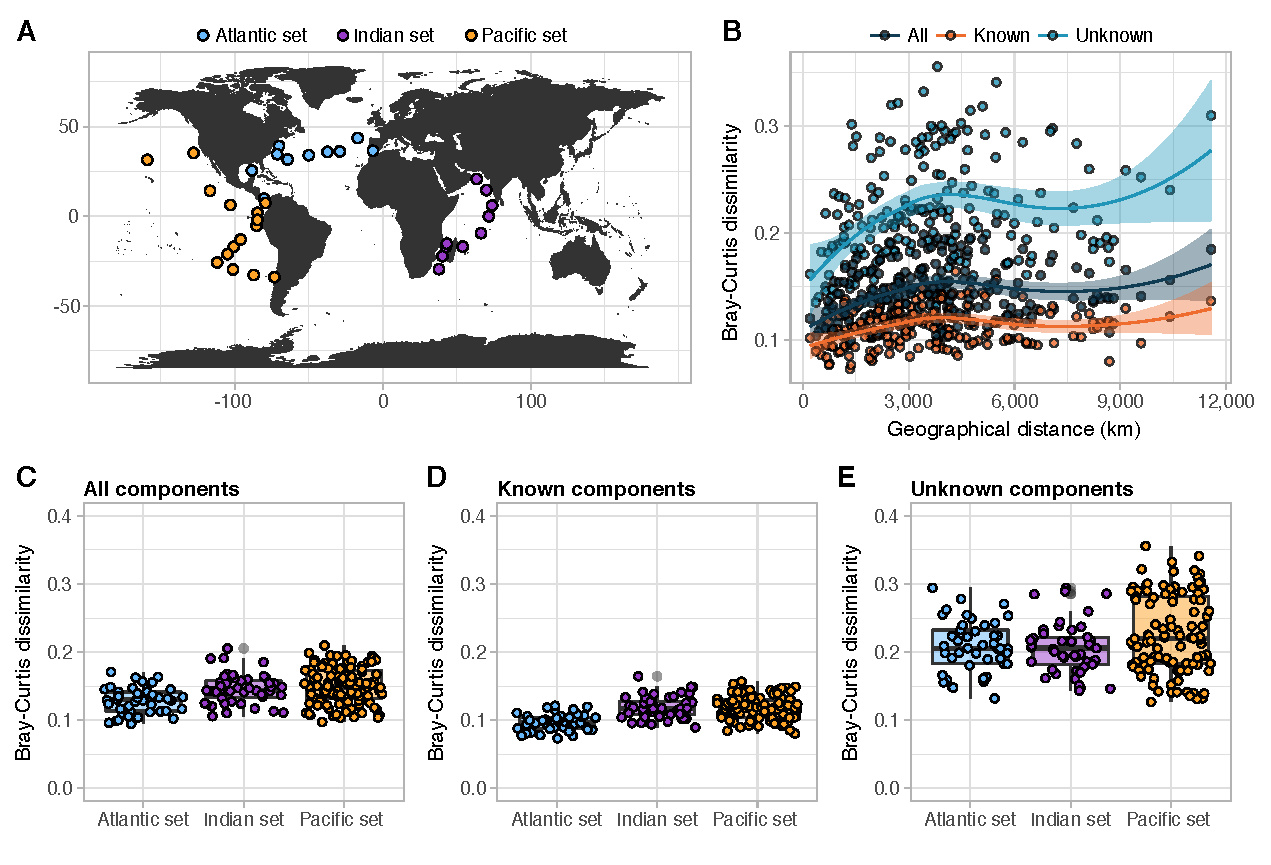
\includegraphics[width=1.0\textwidth] {fig_7}
	\caption{\textbf{Distance-decay analysis}A) Map of TARA Ocean samples used for distance-decay analysis. Samples were divided into regions: Pacific, Atlantic, and Indian. B) Combined distance-decay of samples between all regions. Sites appear three times defined by the Unknowns (EU + GU), Knowns (K + Kwp), and All. The x-axis denotes the geographical distance between sampling sites, while the y-axis denotes the Bray-Curtis dissimilarity beta diversity measurement. (C-E) Box-plots of the pairwise Bray-Curtis dissimilarity beta diversity measurement for each component category, separated by ocean region.}\label{fig7}
\end{figure}

\begin{figure}[h!]
	\centering
	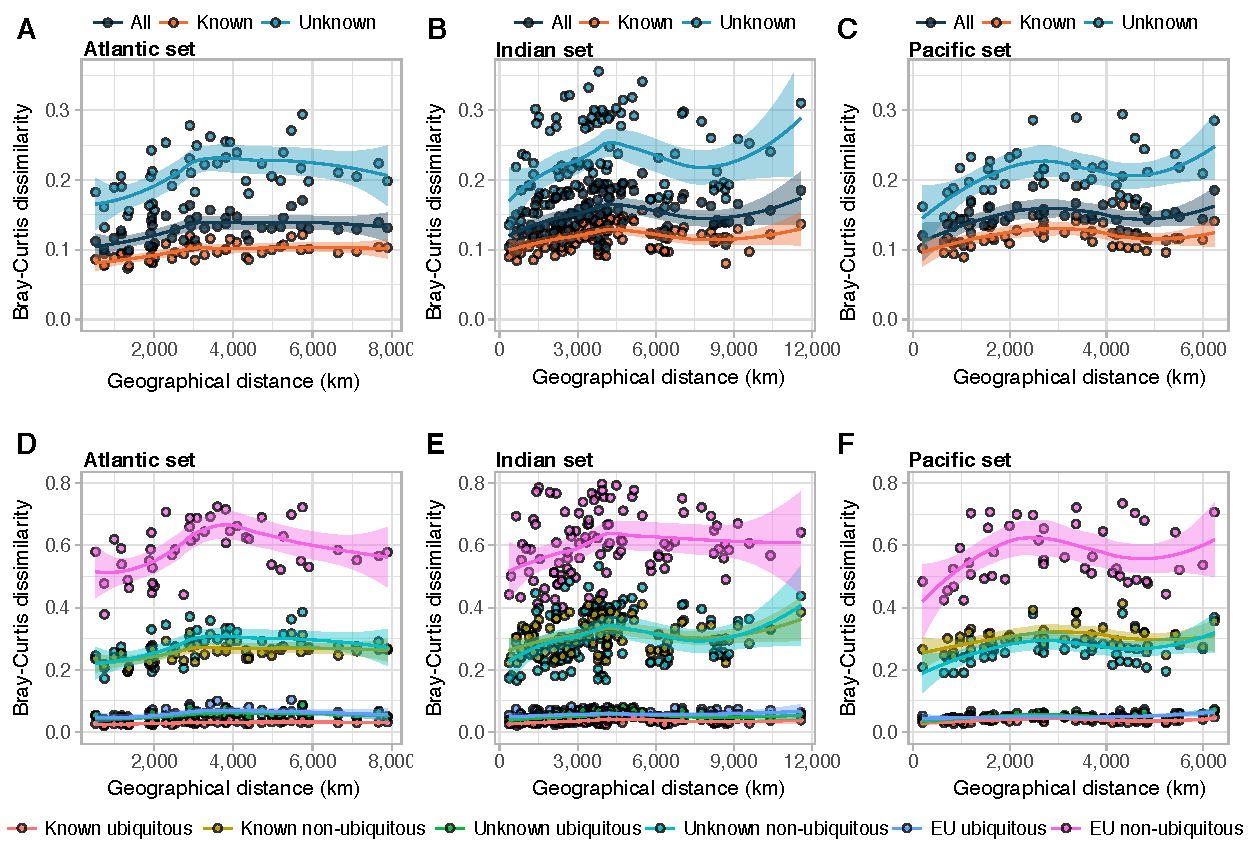
\includegraphics[width=1.0\textwidth] {fig_8}
	\caption{\textbf{Distance-decay, ubiquitous vs. non-ubiquitous}(A-C). Distance-decay plot of TARA ocean surface, prokaryotic metagenomes by oceanic region. Sites appear six times defined by the EU (ubiquitous, non-ubiquitous), GU (ubiquitous, non-ubiquitous), and Knowns (ubiquitous, non-ubiquitous). The x-axis denotes the geographical distance between sampling sites, while the y-axis denotes the Bray-Curtis dissimilarity beta diversity measurement. (D-E) Box-plots of the Bray-Curtis dissimilarity beta diversity measurement for each component category.}\label{fig8}
\end{figure}

On the other hand, the larger Known matrix could have more noise due to its increased component list and be less sensitive to the Known adaptive protein signal, thus decreasing dissimilarity between sites.\\

When sites are defined by the Knowns they are the most similar in all ocean regions. This may be explained by the bias that Known components (Knowns with PFAM annotations) are protein sequences that are shared between a large fraction of the microbial community (e.g. housekeeping genes).\\

The majority of our knowledge of Known microbial functions comes from essential/core gene experiments on cultured microbes that have been studied in the lab \citep{Bernard_2018}. Since our knowledge of protein functions are constrained by this, the Known fraction may be similar in all environments. Additionally, it has been shown that essential/core genes receive less purifying selection and are more conserved across the domains of life \citep{Jordan_2002}. Thus when sites are defined by Known components, dissimilarity is lower due to the overlap of known components between microbes.\\

\begin{table}[]
\centering
\caption{Mantel and Partial Mantel test to measure correlation (spearman) better beta-diversity and Haversine distance of TARA Ocean dataset.}
\label{my-label}
\begin{tabular}{lllll}
\textbf{Component Category}   & \textbf{Mantel statistic (?)} & \textbf{p-value} & \textbf{partial-Mantel} & \textbf{p-value} \\
\textbf{Unknowns (EUs + GUs)} & 0.966                         & 0.001            & 0.512                   & 0.001            \\
\textbf{Knowns (K + Kwp)}     & 0.968                         & 0.001            & 0.509                   & 0.001            \\
\textbf{All combined}         & 0.965                         & 0.001            & 0.515                   & 0.001           
\end{tabular}
\end{table}

On a global scale, the Mantel test showed a significant positive correlation between genetic distance (Bray-Curtis) and geographical distance (Haversine) for the three component classes (Table 8), indicating that closer samples are more similar than the distant. Those results are expected as the geographic isolation is related to the well-defined continental separation of the three oceanic regions used in the analyses: Atlantic, Pacific, and Indian. In all three ocean regions, when sampling sites are defined by All component categories, overall site dissimilarity increases in comparison to the Knowns. This is most likely because including the Unknown fraction in conjunction with the Known fraction increases overall site dissimilarity. The unique, site specific signal from the EUs and GUs may come from the rare biosphere and be environmentally adaptive proteins. This can add site unique component abundances which in turn increase dissimilarity between sites. Additionally, in all three ocean regions, each component category has a similar Bray-Curtis dissimilarity. This results hints that the relationship between the component categories may be a global ocean trend.\\

The All category represents the utilization of an entire metagenomic sample. In general, functional metagenomic analyses only compare ORFs that have known functions while the rest of the unannotated sequences are discarded. These analyses come in the form of heat maps \citep{McMahon_2015} or aggregated ordinations \citep{Louca_2016}. Here, it is demonstrated that incorporating the whole metagenomic sample into beta diversity measurements is informative and helps to highlight the dissimilarities between the samples.\\

Separate analyses were then performed on each individual region. This was done to remove the effect of continental masses distorting the distance decay-analysis, increase resolution of the analysis on the specific regions, and take advantage of the best transects the TARA Ocean sampling regime had to offer.\\

The Atlantic region had samples that transected the North Atlantic Ocean across the Gulf Stream (Fig. 8. B). In Fig. 8 A, there is a peak of dissimilarity in all three component categories at around 3,000 km. Increase in sample dissimilarity between 0 and 3,000 km is most likely due to the changing environment from coastal to open water. The dissimilarity then levels off from 3,000 km to 8,000 km. This could be due to the open water samples being in the Gulf stream. This ocean current pulls warm subtropical waters across the Atlantic towards Europe. The current may maintain similar environmental parameters as it crosses the Atlantic thus removing the distance-decay effect on microbial communities.\\

The Pacific and Indian sample regions had samples that followed a latitudinal North South transect (Fig. 8 B-C). Both distance-decay plots follow a similar trend with an initial positive slope increase in dissimilarity, followed by a trough, then ending with dissimilarity increasing again. Previous findings have shown that environmental variation has more of an effect on functional group composition than dispersal limitation in the open ocean \citep{Louca_2016}. Additionally, temperature has been shown to be the main driving force for community composition in surface ocean waters \citep{Sunagawa_2015}. These observations are congruent with the curvature found in Pacific region distance-decay plot because similar environments can be found on either side of the equator in low or high latitudes. Latitudes equidistant from the equator receive similar solar radiation due to the curvature of the Earth and thus reflect similar temperatures (e.g. Arctic and Antarctic waters).\\



\begin{table}[]
\centering
\caption{Mantel and Partial Mantel test to measure correlation (spearman) between beta-diversity and Haversine distance in local in Atlantic, Pacific, and Indian ocean regions of TARA Oceans.}
\label{my-label}
\begin{tabular}{llllll}
\textbf{Component Category} & \textbf{Metagenomic set} & \textbf{Mantel statistic (?)} & \textbf{p-value} & \textbf{partial-Mantel} & \textbf{p-value} \\
\textbf{Unknowns (EU + GU)} & Atlantic & 0.385 & 0.0201 & 0.0201 & 0.0240 \\
\textbf{Knowns (K + Kwp)} & Atlantic & 0.475 & 0.0066 & 0.387 & 0.0240 \\
\textbf{All combined} & Atlantic & 0.433 & 0.0120 & 0.417 & 0.0173 \\
\textbf{Unknowns (EU + GU)} & Pacific & 0.128 & 0.2528 & 0.086 & 0.3160 \\
\textbf{Knowns (K + Kwp)} & Pacific & 0.072 & 0.3384 & 0.046 & 0.3818 \\
\textbf{All combined} & Pacific & 0.111 & 0.2630 & 0.076 & 0.3317 \\
\textbf{Unknowns (EU + GU)} & Indian & 0.068 & 0.3189 & 0.068 & 0.3070 \\
\textbf{Knowns (K + Kwp)} & Indian & -0.196 & 0.8849 & -0.177 & 0.8595 \\
\textbf{All combined} & Indian & -0.013 & 0.5159 & -0.013 & 0.5159
\end{tabular}
\end{table}

\begin{figure}[h!]
	\centering
	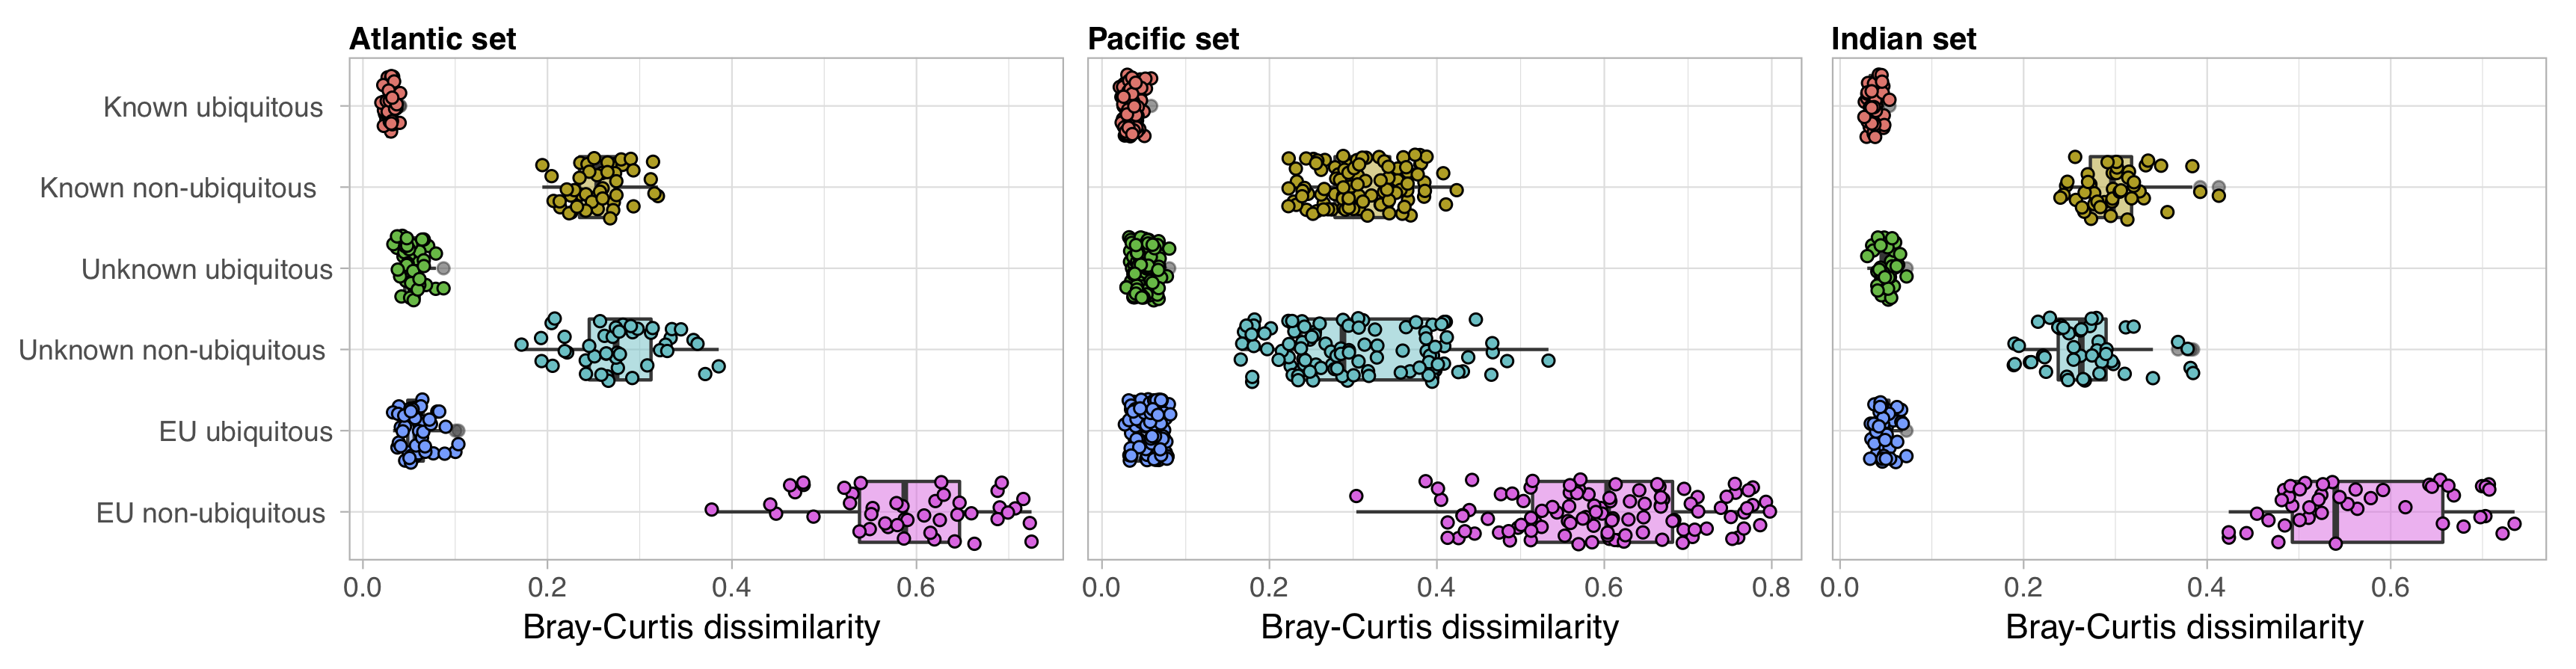
\includegraphics[width=1.0\textwidth] {fig_9}
	\caption{\textbf{Beta-diveristy of ubiquitous vs on-ubiquitous components} (A-C) Distance-decay plot of TARA ocean surface, prokaryotic metagenomes by oceanic region. Sites appear six times defined by the EU (ubiquitous, non-ubiquitous), GU (ubiquitous, non-ubiquitous), and Knowns (ubiquitous, non-ubiquitous). The x-axis denotes the geographical distance between sampling sites, while the y-axis denotes the Bray-Curtis dissimilarity beta diversity measurement. (D-E) Box-plots of the Bray-Curtis dissimilarity beta diversity measurement for each component category.}\label{fig9}
\end{figure}

Another explanation for the distance-decay curvature that can be applied to both the Indian and Pacific regions is the sampling regimes moving away and back towards the coasts. Since the sampling paths start and return in similar environments across the gradient of open to coastal waters, component composition dissimilarity increases and decreases, responding to the environment. Though the Atlantic has a similar sampling structure, the Indian and Atlantic have a higher density of coastal samples. Both the Indian and Pacific distance-decay analysis have increases in dissimilarity at the farther geographic distances in the plot. This may be explained by the influence of the coastal environments selecting for unique component composition due to terrestrial runoff. 

To further investigate if the Unknowns are site specific and adaptive proteins, component categories were separated and filtered into ubiquitous and non-ubiquitous fractions. The requirement for being ubiquitous was having a presence in every TARA ocean surface sample, anything less was considered non-ubiquitous. In all three ocean regions similar patterns emerge. When sites are defined by non-ubiquitous categories, EU defined sites are significantly more dissimilar than the other non-ubiquitous categories (Fig. 9). The Unknown and Known non-ubiquitous categories fall within a similar range of dissimilarity. On the other hand, the categories defined by ubiquitous fraction all fall into a very low, similar dissimilarity range of little no distance decay (Fig. 9).

The EU non-ubiquitous sites were overall the most dissimilar to each other. In light of the results from the ordination, and niche breadth analysis, this was an expected result. EUs have shown to be site specific, and are likely adaptive proteins. Removing the EU ubiquitous fraction that is found everywhere increases the site specific, adaptive signal even more, thus making sites more dissimilar. The non-ubiquitous EU fraction most likely drives the overall dissimilarity between sites when the entire metagenomic sample is taken into account.\\

The non-ubiquitous components all follow a similar distance-decay trend to their combined component analysis. This makes sense because non-ubiquitous components have a higher chance of being inherently adaptive because they are not found everywhere. In light of this, the non-ubiquitous fraction is most likely driving the distance-decay trends we observe.\\

When the ubiquitous fraction is removed from the Unknowns and Knowns their beta-diversity dissimilarities converge, and in the case of the Pacific and Indian region, overlap. This overlap in similarity is more than likely due to the similarity of the Kwp and GU component categories. GUs are taxonomically characterized in sequencing databases similar to Kwp but lack a functional annotation. On the scale of functional characterization, GUs and Kwp are the most similar by definition in the Vanni et. al. workflow. Due to their similarity within the design of the functional categories, they may have similar biogeographical patterns in the oceans. Another explanation is that the non-ubiquitous Knowns provide a more site specific, adaptive signal and drive dissimilarity to be more similar to the non-ubiquitous GUs. The niche breadth analysis showed that the Knowns have a similar distribution of narrow to wide B components. By removing the ubiquitous fraction, the narrow B components increase in relative abundance and thus drive the increase in dissimilarity.\\

The Unknowns may represent a hybrid of both ?core? and environmentally adaptive proteins. The unknown ubiquitous fraction was making the unknown defined sites more dissimilar. There is a possibility that ubiquitous clusters could be involved in niche adaptation. It has been shown that core genes can be adaptive for the sugar metabolism in the metapangenome of \textit{Prochlorococcus} \citep{Delmont_2018}. Additionally, \cite{Delmont_2018} demonstrated that the accessory pangenome can be made up of environmental core and environmental accessory genes. This was determined by mapping metagenomic reads to the Prochlorococcus and seeing in how many genomes the reads occurred. If an ORF is part of the core genome, then there may be a higher possibility that the protein is ubiquitous.\\

The ubiquitous fraction of every component category all followed a similar trend of defining sites as extremely similar with no significant distance decay. In other words, this group of components are found in every sample of the global regions analyzed and have a similar dissimilarity signal regardless of distance. These results were expected for the Knowns and possibly the GUs, but were surprising to see for the EUs. Known components contain a lot of housekeeping and essential functions (i.e. shared between all prokaryotes), thus a strong and similar ubiquitous signal is to be expected. On the other hand, EUs have been shown to have a small niche breadth and be adaptive responses to the environment. The signal of ubiquitous EU components, which have no functional annotation or are found in sequenced or draft genomes, is not in line with the previous results in this thesis. This may demonstrate that the EUs share core microbial functions with the other component categories in the world's oceans. This is a surprising results because it could infer that a set of proteins from a ubiquitous domain of life and or function in the ocean have been left uncharacterized by metagenomics. In total, 6,587 EUs are in this category and were subjected to further investigation. \\

\textbf{Investigating the Ubiquitous EU fraction}\\

To demonstrate that the ubiquitous EU fraction is a legitimate functional signal, we took steps to remove spurious proteins and to detect distant homology and taxonomy. First we ran antiFAM HMMERs against the potential EU sequences. This removed 250 spurious proteins from the component set. Next, HHblits detected distant homology in 4,823 of the potential EUs with 3,811 having their best hit being a Hypothetical or uncharacterized protein. Finally, for the EUs that were not hit by HHblits we assigned taxonomy using Kaiju, 81 EUs were classified. This left us with 1514 potential EUs with no distant homology or taxonomy.\\

HHblits iteratively compares one HMM against another HMM to detect distant homologies. HMM vs HMM is the most effective technique for detecting distant homologs because it can detect the similarity of the structural templates that usually diverge slower than the sequences themselves. Proteins may remain structurally very similar long after their sequence similarity has been lost. The fact that HHblits was able to detect distant homology in 4823 EUs indicates that some of the Vanni et. al. EU components may in fact be GUs. This caveat has been solved in the upcoming version of the workflow (Vanni et. al. in prep). HHblits did however fail to detect distant homology in the 1514 ubiquitous EUs. This was either because they are truly novel, or simply an artifact of sequencing or assembly.\\

\begin{table}[]
\centering
\caption{Kaiju taxonomic annotation of ubiquitous potential EUs with no distant homology}
\label{my-label}
\begin{tabular}{ll}
\textbf{Kaiju taxonomic assignment} & \textbf{Number of ubiquitous EUs} \\
\textbf{Bacteria} & 64 \\
\textbf{Eukaryota} & 3 \\
\textbf{Environmental} & 14 \\
\textbf{Total} & \textbf{81}
\end{tabular}
\end{table}

We used Kaiju with the objective to gather taxonomic information of the ubiquitous EUs using a k-mer based approach that in theory is less database biased. The tool takes advantage of the fact that different taxa have different amino acid compositions signatures.\\

\begin{table}[]
\centering
\caption{6,587 ubiquitous EUs were identified in the distance-decay analysis. These were the steps taken to ensure the ubiquitous EUs are indeed protein coding sequences.}
\label{my-label}
\begin{tabular}{ll}
\textbf{Ubiquitous EU classification step} & \textbf{Number of ubiquitous EUs} \\
\textbf{Removed with antiFAM} & 250 \\
\textbf{HHblits distant homology detected} & 4823 \\
\textbf{Kaiju taxonomy classified} & 81 \\
\textbf{Potential EU} & \textbf{1433}
\end{tabular}

This strategy is unique compared to other more traditional nucleotide methods like Kraken \citep{Wood_2014}. Thus, the Kaiju hits only imply there is a similar k-mer frequency between the 81 Kaiju hits and any of the taxa on NCBI nr database. \\
Kaiju did not detect taxonomy in all of the ubiquitous EUs. This may have occurred for a few reasons. First, some ubiquitous EUs may be a new expansion of the tree of life, similar to the Candidate Phyla Radiation \citep{Danczak_2017}, and thus have a unique k-mer frequency. Second, they are sequencing artifacts and errors, thus have a random, non-related k-mer frequency to known taxa. A future direction for the Vanni et. al. workflow could be to add tool Spurio to the cluster validation steps to identify and remove spurious genes \citep{H_ps_2018}. \\

In light of ubiquitous vs non-ubiquitous genes, the discussion of ?core? or ?essential? microbial functions can be brought up. The current understanding of ?core? genomic functions and metabolic pathways is heavily biased by the low number of deeply characterized microbes grown in the lab \citep{Prosser_2014}. The core functions found in common in laboratory isolate may not be representative of the total environmental ?core?. The Ubiquitous EUs may be a new ?core? set of genes that have only been detected by means of environmental gene content comparison. \\

\textbf{Mapping EUs to TARA Ocean MAGs}\\

The onset of techniques to extract metagenomic assembled genomes (MAGs) from metagenomic samples has allowed for great insight into microbial populations. Deeper sequencing technology, allowing for 50x of less abundant microbial populations, and efficient differential coverage binning algorithms has led to an era of Metagenomics 2.0 \citep{McMahon_2015}. Additionally, MAGs can now be manually curated in an efficient manner leading to higher quality \citep{Eren_2015}. Although MAGs represent populations of similar microbes and are not complete genomes, the binned contigs are a step closer to the genetic units they came from, genomes. EUs that successfully mapped to the \cite{Delmont_2017}  MAGs were then upgraded to a new category of the unknown, Population Unknowns.\\

\textbf{Population Unknowns (PU)}\\
ORF clusters with an unknown function but map to contigs in MAGs. 

As a final confirmation to determine if the ubiquitous EU components are indeed real proteins found in the environment, we mapped the clusters belonging to the selected components against a set of high quality metagenomic assembled genomes binned from the TARA Ocean prokaryotic dataset \citep{Delmont_2017}. Finding ubiquitous EUs in MAGs from the environment they originated from increases the chance of the component being indeed a real environmental protein sequence because it is occurring in the context of a population of similar genomes in the environment. \\

\begin{figure}[h!]
	\centering
	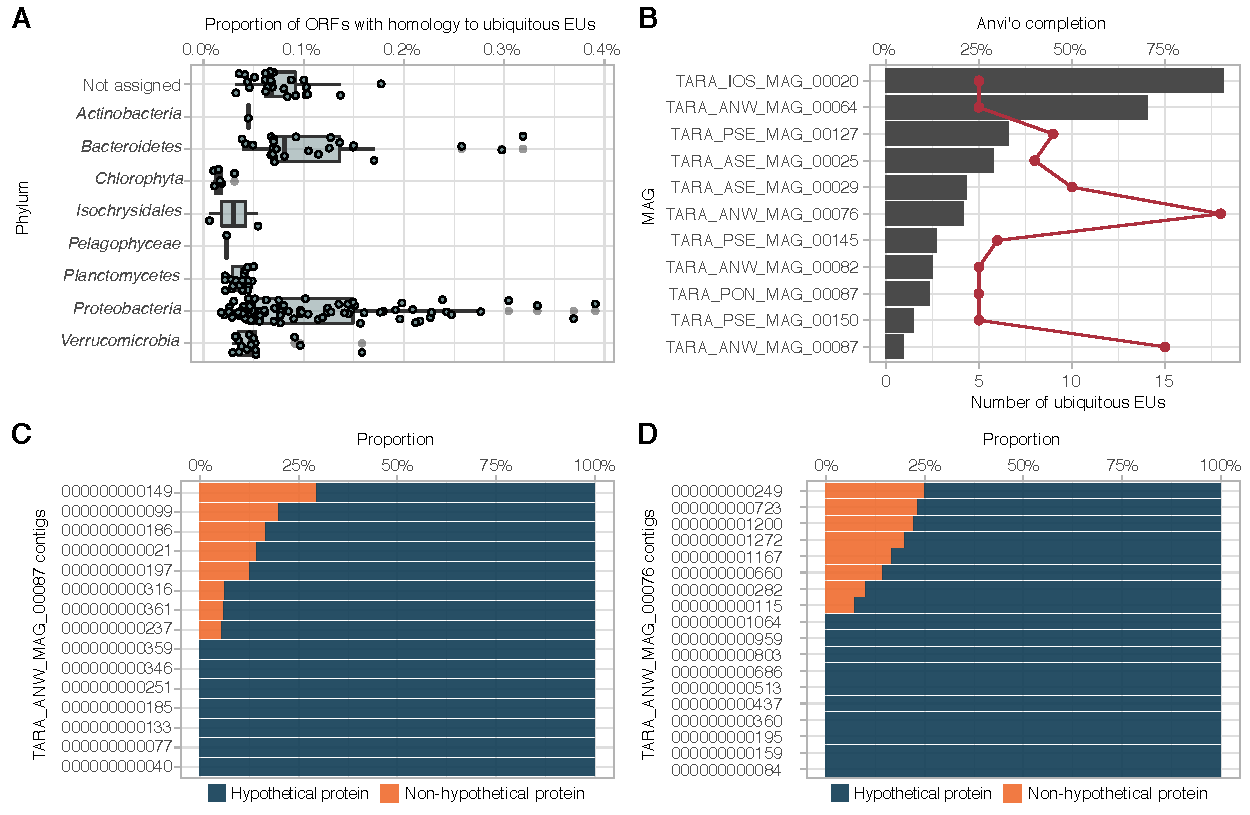
\includegraphics[width=1.0\textwidth]{fig_10}
	\caption{\textbf{EU mapping results}}\label{fig10}
\end{figure}

Out of the 957 non-redundant MAGs, the ubiquitous EUs mapped to 178 of them. This is a significant amount of the MAGs. If the potential origin of the ubiquitous EUs is from organisms that are part of the rare biosphere, this means that the TARA Ocean project sampled at a critical moment when the rare microbes ?bloomed? due to perfect environmental conditions \citep{Gobet_2011}. . In order to be binned into MAGs, there has to be enough sequencing depth and coverage of the population. Continual deep sequencing of marine waters is needed to catch more of the rare biosphere for metagenomic assembly and expand our knowledge of the world oceans. 
Our next goal was to examine the genomic neighborhood of the ubiquitous EUs on the contig of which they mapped to. Investigating the genomic neighborhood can lead to the inference of a possible function of the EU. Furthermore, if the EU is surrounded by genes of known function, this adds clarity that the EU is a part of a real contig and possibly an operon.\\

To select which MAG contig to visualize, we picked the MAGs with the least completeness and highest number of ubiquitous EUs mapped to it (Fig. 10B). Next we selected contigs to visualize by choosing the ones with the highest proportion of non-hypothetical proteins (Fig. 10 C-D). The more annotated proteins on the contig, the more genomic context we can apply to the ubiquitous EU. \\

TARA ocean MAGS TARA\_ANW\_MAG\_00076 and TARA\_ANW\_MAG\_00087 were selected for contig analysis because they were the most enriched with ubiquitous EUs (Fig 10B). These mags originated from the South West Atlantic Ocean TARA sampling sites. We then picked contigs where the ubiquitous EUs mapped to and arranged them based on content of non-hypothetical genes (Fig 10 C-D). This was in order to have a higher chance of having the ubiquitous EU surrounded by genes of known function. If the ubiquitous EU is surrounded by genes of known function, it adds another layer of evidence that the EU is indeed a real sequence. If the EU was spurious, multiple levels of the metagenomic analysis to make the MAG would have had gone wrong including gene prediction, assembly and binning.  \\

\begin{figure}[h!]
	\centering
	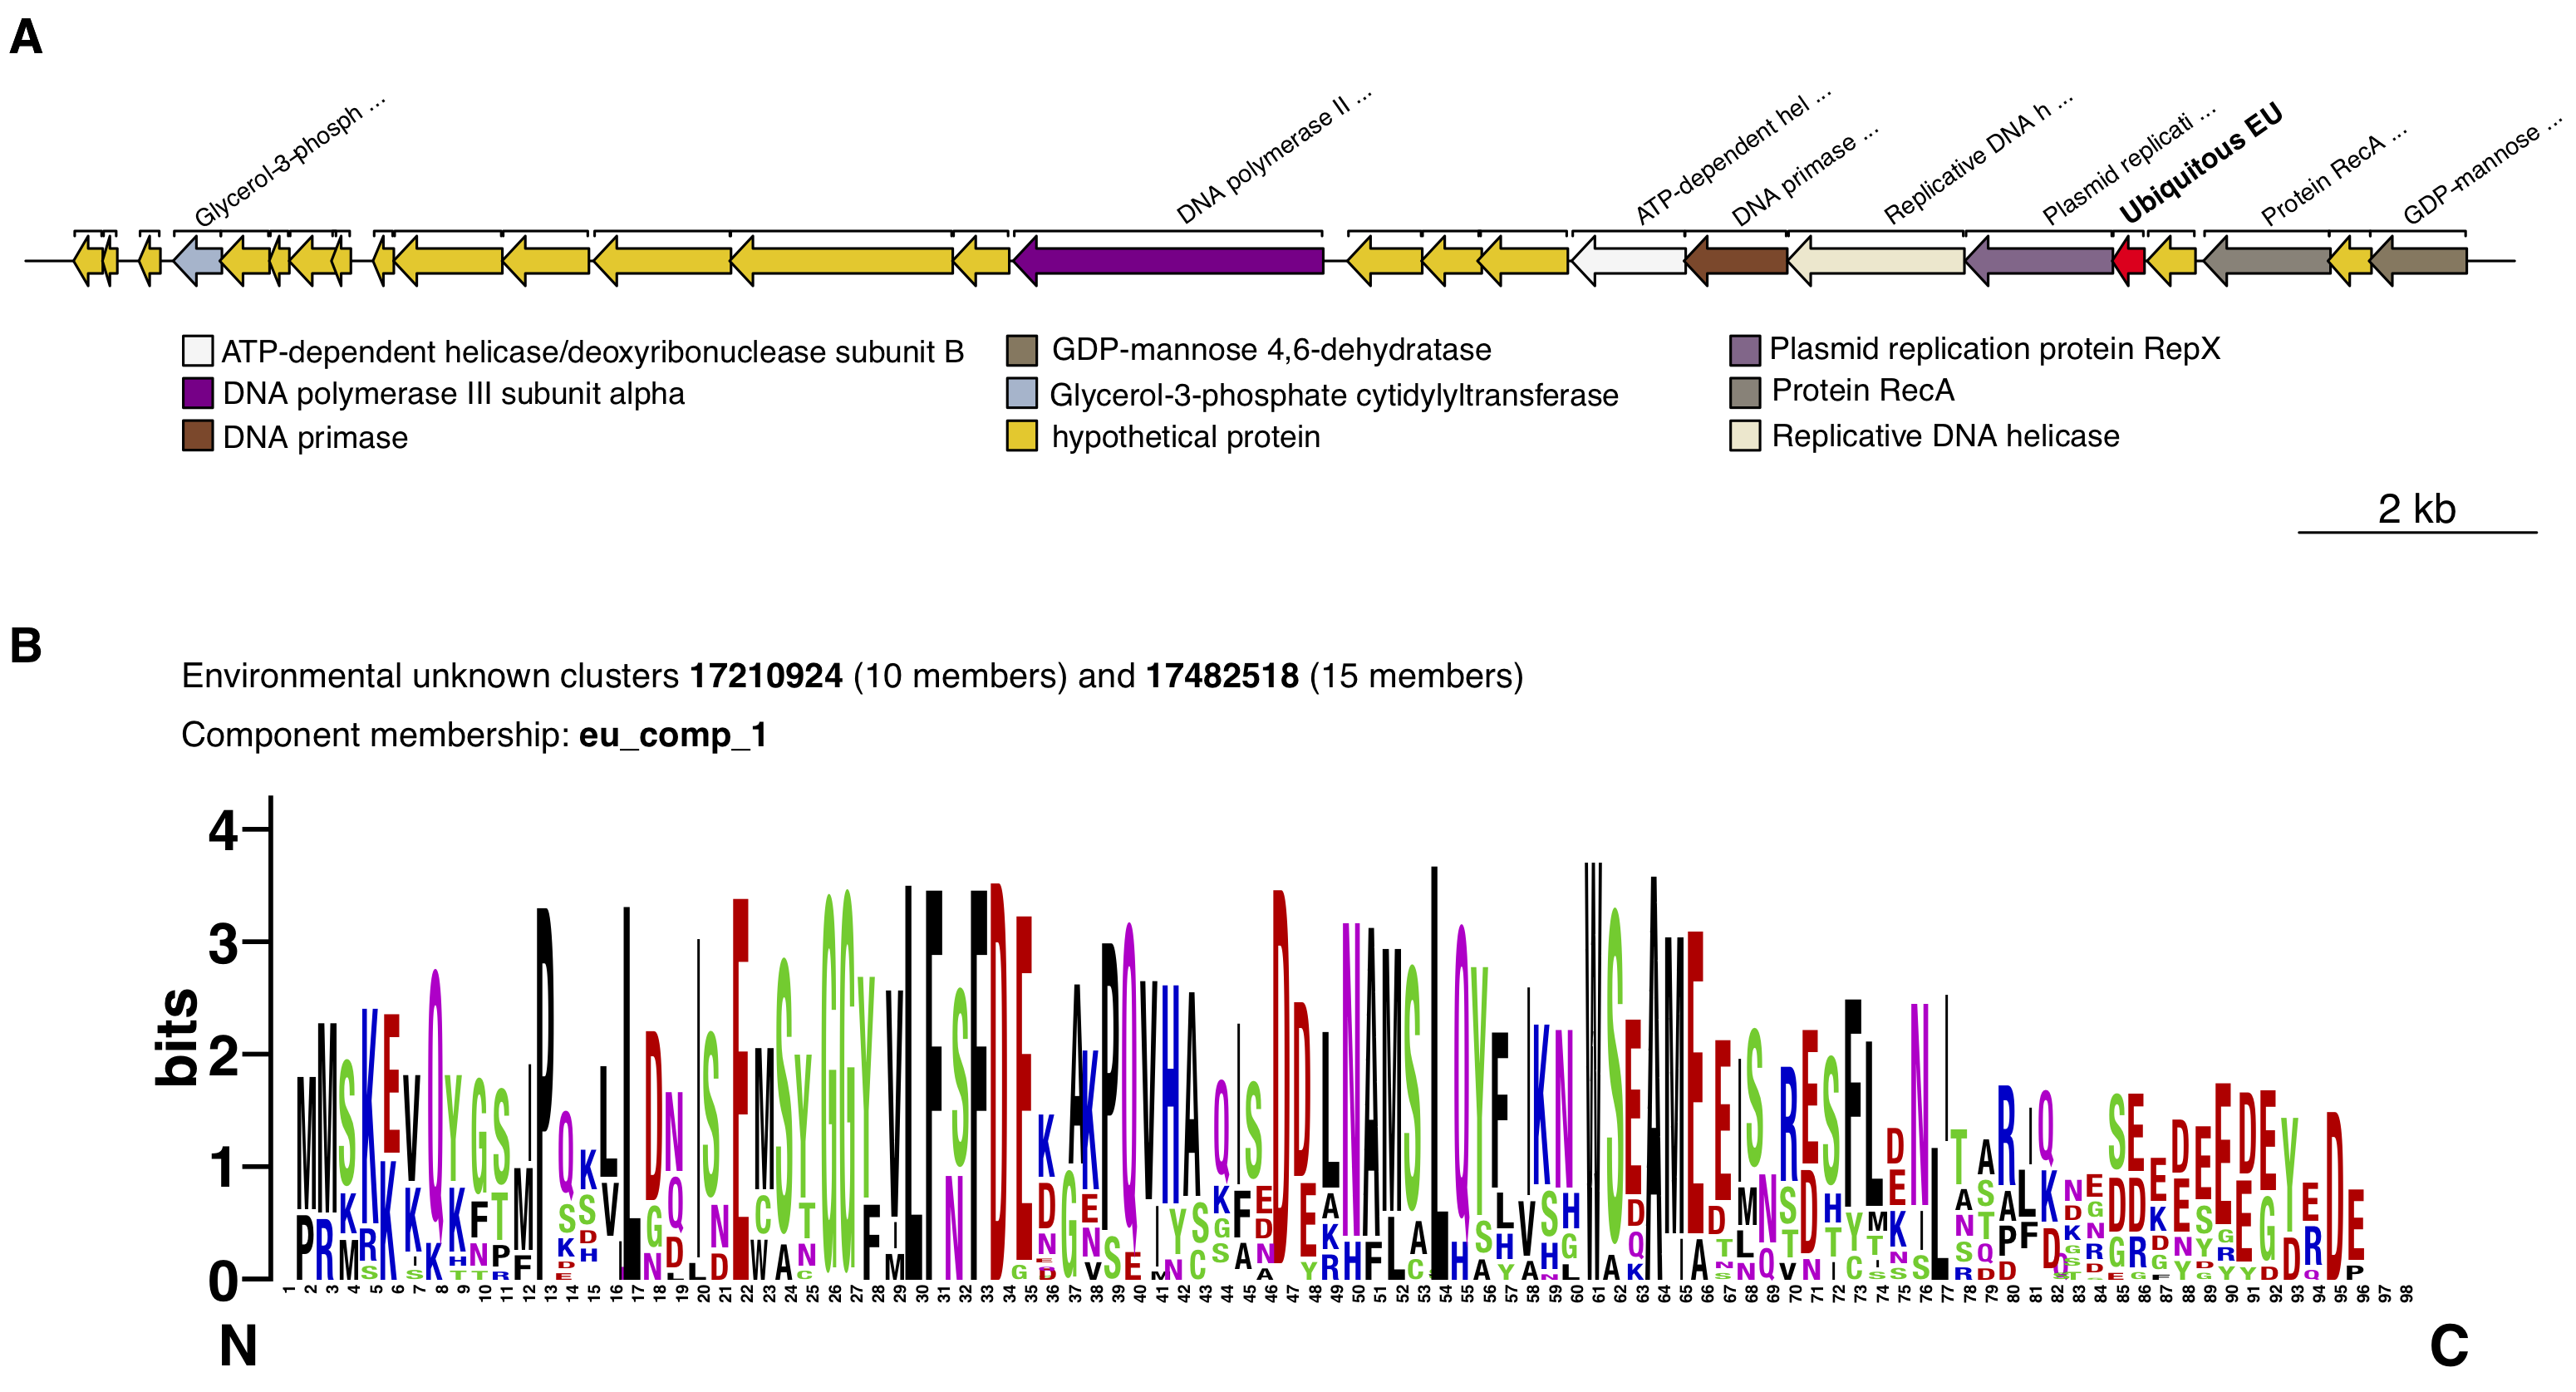
\includegraphics[width=1.0\textwidth] {fig_11}
	\caption{\textbf{EU gene visualization}}\label{fig11}
\end{figure}


In Figure 11 A, contig TARA_ANW_MAG_00087_000000000149 is shown. Highlighted in red, is the predicted ORF with significant homology Environmental Unknown clusters  (17210924 and 17482518) members of the ubiquitous EU component eu_comp_1. Within its genomic neighborhood are genes relating to DNA and plasmid replication and repair including DNA polymerase II, DNA primase, and protein RecA. Gene placement in prokaryotic genomes is not random. Genes are grouped together to increase transcriptional efficiency to respond to stimuli in the environment. The lac operon is an example of a group of genes that are transcribed together to metabolize lactose. Since this ubiquitous EU is associated with these DNA and plasmid repair genes, we can hypothesize that it has a related function. Another aspect to consider is that the surrounding genes are essential/core functions for microbial life. Without DNA repair mechanisms, genetic integrity of species would not be able to be maintained. Considering that the ubiquitous EU is surrounded by essential ?ubiquitous? biological functions and its found in every sample in the TARA Ocean dataset, there is a higher chance this is a real protein. Furthermore, the consensus amino acid residues after aligning all sequences from both clusters belonging to the component eu_comp_1 (Fig. 11B) contain ?2 active residues (E, D), one of the conditions defined to identify non-spurious ORFs by \cite{Li_2008}, , supporting one more time that the ORF might be real. The ubiquitous EUs that were not found in the MAG data set or detected for distant homology have the potential of being part of the genomic repertoire of members present in the rare biosphere. There is mounting evidence that the theory in microbial ecology that ?everything is everywhere? but is selected for by the environment is indeed true \citep{Gibbons_2013}. All ocean samples may contain a ?microbial seed bank? where many rare taxa exist in stationary phase or grow extremely slowly \citep{ Pedros_2006}. This theory has mainly been investigated via 16S rDNA amplicon sequencing because the scientific question was focused on phylogenetic diversity. With deeper sequencing, immense diversity of low abundance microbes have been recovered. New protein families have been detected before via mass sequencing efforts and protein clustering \citep{Yooseph_2007}.. The difference made in this analysis was the Unknown fraction was put in a functional biogeographical context. Due to the deep metagenomic sequencing of the TARA ocean dataset, this maybe the first time that ?core? functions from the rare biosphere have been revealed. Due to the Vanni et. al. Unknown cluster categories, the unannotated protein diversity of the TARA ocean data set was able to be accounted for.\\

